\documentclass{beamer}
\mode<presentation> {
%\usetheme{Dresden}
\usetheme{CambridgeUS}
}
\newcommand{\subitem}{\par\qquad}
\usepackage{booktabs}

\usepackage{tikz}
\usepackage{subfigure}	
\usepackage[round]{natbib}   % omit 'round' option if you prefer square brackets
\DeclareMathOperator*{\argmin}{argmin}
\DeclareMathOperator*{\argmax}{argmax}

\newcommand{\independent}{\mbox{${}\perp\mkern-11mu\perp{}$}}
\newcommand{\notindependent}{\mbox{${}\not\!\perp\mkern-11mu\perp{}$}}
\newcommand{\iid}{\overset{\text{iid}}{\sim}}
\newcommand\indeptest[2]{\mathtt{TestIndependence}(#1,#2)}
\newcommand\residuals[2]{\mathtt{FittedNoise Values}(#1,#2)}
%\newcommand{\C}[1]{\mathcal{#1}}
\newcommand{\B}[1]{\mathbf{#1}}
\newcommand{\prob}{{\mathbb P}}
\newcommand{\R}{{\mathbb R}}
\newcommand{\RN}{{\mathbb R}}
\newcommand{\Z}{{\mathbb Z}}
\newcommand{\N}{{\mathbb N}}
\newcommand{\X}{{\mathbf X}}
\newcommand{\Y}{{\mathbf Y}}
\newcommand{\x}{{\mathbf x}}
\newcommand{\e}{{\mathbf e}}
\newcommand{\n}{{\mathbf n}}
\newcommand{\SE}{\C{S}}
\newcommand{\graph}{{\mathbf{graph}}}

\newcommand{\onemat}[0]{{\mathbf 1}}
\newcommand{\cV}{{\cal V}}
\newcommand{\cX}{{\cal X}}
\newcommand{\cP}{{\cal P}}
\newcommand{\cY}{{\cal Y}}
\newcommand{\cA}{{\cal A}}
\newcommand{\cB}{{\cal B}}\newcommand{\cL}{{\cal L}}
\newcommand{\cW}{{\cal W}}
\newcommand{\cI}{{\cal I}}
\newcommand{\cD}{{\cal D}}
\newcommand{\cF}{{\cal F}}
\newcommand{\cC}{{\cal C}}
\newcommand{\cR}{{\cal R}}
\newcommand{\HSIC}{{\mathrm{HSIC}}}
\newcommand{\dep}{{\mathrm{DEP}}}
\newcommand{\s}{{{\mathbf s}}}
\newcommand{\cH}{{\cal H}}
\newcommand{\cG}{{\cal G}}
\newcommand{\cS}{{\cal S}}
\newcommand{\cT}{{\cal T}}
\newcommand{\tl}{\tilde}
\newcommand{\T}{{\cal T}}
\newcommand{\E}{{\cal E}}

\newcommand{\ifmoclin}{{IFMOC$_\mathrm{lin}$ }}
\newcommand{\ifmocgp}{{IFMOC$_\mathrm{GP}$ }}
%\newcommand{\ffmoc}{{$\C{F}$-FMOC}}
%\newcommand{\ffmo}{{$\C{F}$-FMO}}
%\newcommand{\Gp}{\C{G}'}
%\newcommand{\G}{\C{G}}
\newcommand{\Gc}{\C{G}_c}
\newcommand{\mean}{{\mathbf E}}  
\newcommand{\var}{{\mathbf{var}}}  
%\newcommand{\var}{{\mathbb{V}\mathrm{ar}}}  
\newcommand{\eps}{{N}}  
\newcommand{\PA}[2][]{{\B{PA}}^{#1}_{#2}}
\newcommand{\tPA}[2][]{{\tilde{\B{PA}}}^{#1}_{#2}}
\newcommand{\CH}[2][]{{\B{CH}}^{#1}_{#2}}
\newcommand{\DE}[2][]{{\B{DE}}^{#1}_{#2}}
\newcommand{\ND}[2][]{{\B{ND}}^{#1}_{#2}}
\newcommand{\eref}[1]{(\ref{#1})}
\newcommand{\given}{\,|\,}
\newcommand{\abs}[1]{\left|#1\right|}
\newcommand{\supnorm}[1]{\lVert#1\rVert_\infty}
\newcommand{\norm}[1]{\left\Vert{#1}\right\Vert\,}
\newcommand{\supp}{{\mathrm{supp}\,}}
% \newcommand{\argmax}{{\mathrm{argmax}\,}}
% \newcommand{\argmin}{{\mathrm{argmin}\,}}
\newcommand{\im}{\mathrm{Im}}
\newcommand{\DM}{\mathrm{DM}}
\newcommand{\tn}{{\tilde{n}}}
\newcommand{\paxi}{{\bf x}_{\mbox{pa}(i)}}
\newcommand{\dd}{{\partial }}
\newcommand{\dx}{{\partial x}}
\newcommand{\dy}{{\partial y}}
\newcommand{\btheta}{{\bf \theta}}
\newcommand{\easy}{$\bullet$}                   %easy problem
\newcommand{\law}[1]{\mathcal{L}({#1})}
\newcommand{\lawX}{{\law{\mathbf X}}}
\newcommand{\lawn}[1]{\mathcal{L}_n({#1})}
\newcommand{\lawN}{{\law{\mathbf N}}}
\newcommand{\llaw}{{\mathbf{law}_X}}
\newcommand{\todo}[1]{{\color{red} TODO: {#1}}}
\newcommand{\Lequ}{\overset{\mathcal{L}}{=}}
\newcommand{\SEM}{SEM }
\newcommand{\DAG}{DAG }
\newcommand{\SEMs}{SEMs }
\newcommand{\DAGs}{DAGs }
\newcommand{\tc}{\gamma}
\newcommand{\td}{\delta}
\newcommand{\tnu}{\tilde \nu}

\title[Additive Noise Models]{Additive Noise Models: Identifiability Theorems, Learning Algorithms, Hidden Variables and Time Series} 

\author{Behrad Moniri}
\institute[EE @ Sharif] 
{
Sharif University of Technology \\
\medskip
\textit{bemoniri@ee.sharif.edu}
}
\date{}
\titlegraphic{
\includegraphics[width=2cm]{logo.png}\hspace*{-9.75cm}~%
%	
\includegraphics[width=2cm]{logo.png}
}
\newcommand{\bigCI}{\mathrel{\text{\scalebox{1.07}{$\perp\mkern-10mu\perp$}}}}
\begin{document}
\section{EE-25570 Causal Inference}
\subsection{Presentation of the Final Course Project}
\begin{frame}
\titlepage
\end{frame}
\section{Model Definition}
\begin{frame}
\frametitle{Model Definition}
We call the SCM, C, an addtive noise model if each observed variable
$X_j$ is associated with a node $j$ in a directed acyclic graph G, and the value of
$X_j$ is obtained as a function of its parents in G, plus independent additive noise
$N_j$, i.e.
\begin{equation} \label{eq:anm}
X_j = f_j(\PA{j}) + N_j\,, \qquad j=1, \ldots, p
\end{equation}
with jointly independent variables $N_j$. We will assume that the noise variables have strictly positive density.

\begin{alertblock}{Causal Minimality}
For those models with strictly positive density, causal minimality reduces to the condition that each function $f_j$ is not constant in any of its arguments.
\end{alertblock}
\end{frame}


\section{Identifiability}
\subsection{Bivariate Case}

\begin{frame}
\frametitle{Identifiability: The Bivariate Case}
 \cite{hoyer} proves the following theorem about the identifiability of  bivariate additive noise models.
\begin{theorem}
\begin{small}
An additive noise model with two variables, i.e., $X_1 = N_1$ and $X_2 = f(X_1) + N_2$, with $N_1 \bigCI N_2$, is identifiable if it does not solve the following differential equation for all $x_i,x_j$ with $\nu''(x_j-f(x_i))f'(x_i)\neq 0$:

\begin{equation*}
\begin{split}
\xi'''=   \xi''  \left(-\frac{\nu'''f'}{\nu''}
+\frac{f''}{f'}\right) 
-2 \nu''f''f' %\notag\\
%&\qquad \qquad \qquad 
+\nu'f'''+\frac{\nu'\nu'''f''f'}{\nu''}-\frac{\nu'(f'')^2}{f'}\,,
\end{split}
\end{equation*}
Here $\xi:=\log p_{X_1}$ and $\nu:=\log p_{N_2}$ and we have skipped the arguments $x_2-f(x_1)$, $x_1$, and $x_1$  for $\nu$, $\xi,$ and $f$ and their derivatives, respectively.
\end{small}
\end{theorem}\end{frame}
%------------------------------------------------

\begin{frame}
\begin{corollary}{Gaussian Noise:}
\begin{small}
Assume that $\nu'''= \xi''' = 0$ everywhere. If a backward model exists, then $f$ is linear.
\end{small}
\end{corollary}
\begin{corollary}
\begin{small}
Assume that $f(x) = −x$ and $p_x(x) = e^{-x-e^{-x}}$ and $p_n(n) = e^{-n-e^{-n}}$.
With $p_y(y) = e^{-y-2 \log(1 + e^{−y})}$, $\tilde{p}_n(\tilde{n}) = e^{-2\tilde{n}-e^{-\tilde{n}}}$ and $g(y) = \log(1+e^{-y})$, one obtains:
$$p(x,y) =p_n(y-f(x))p_x(x) =\tilde{p}_n(x-g(y))p_y(y)$$
so the model is not identifiable.
\end{small}
\end{corollary}
\end{frame}
%------------------------------------------------
\subsection{Multivariate Case}
\begin{frame}
\frametitle{Identifiability: From Bivariate to Multivariate}
\begin{definition} \label{def:wnn}
	Consider an ANM with $p$ variables. We call this SCM a \emph{restricted additive noise model} if for all $j \in \B{V}$, $i \in \PA{j}$ and all sets  $\B{S} \subseteq \B{V}$ with  $\PA{j} \setminus \{i\} \subseteq \B{S} \subseteq \ND{j} \setminus \{i,j\}$, there is an $x_{\B{S}}$ with $p_{\B{S}}(x_{\B{S}}) > 0$, such that
	\begin{equation*}
	\Big(f_j(x_{\PA{j}\setminus \{i\}}, X_i), P(X_i \given X_{\B{S}}=x_{\B{S}}), P(N_j)\Big)
	\end{equation*}
	satisfies the bivariate identifiability conditions.
	
	We assume that the noise variables to have non-vanishing densities and the functions $f_j$ are three times differentiable.
\end{definition}
\end{frame}

\begin{frame}
\cite{continous} proves a very interesting theorem. This theorem states how we can generalize a bivariate identifiability to the multivariate case, in this case ANM identifiability.
\frametitle{Identifiability: The Multivariate Case}
\begin{theorem}
	 Let $X_1, \ldots, X_p$ be generated by a restricted additive noise model with graph $G_0$ and assume that $P_\mathbf{X}$ satisfies causal minimality with respect to $G_0$, i.e., the functions $f_j$ are not constant. Then, $G_0$ is identifiable from the joint distribution.
\end{theorem}
\end{frame}
\subsection{PNL}
\begin{frame}
\frametitle{Identifiability: Post Non Linear (PNL) Models}
\begin{definition}
PNL Models are introduced in \cite{postnonlinear}. A PNL is an SCM where each expresses each variable $X_i$ as
$$X_i=g_i(f_i(\PA i) +N_i),\;\;\;  i= 1, ..., n$$
\end{definition}
\end{frame}

\begin{frame}
\begin{theorem}[Bivariate Identifiability]
\begin{small}
Assume that $x_2 = f_2(f_1(x_1) + e2) \;\;\mathrm{and} \;\;x_1 = g_2(g_1(x_2) + e1)$.
 Densities and nonlinear functions are three times differentiable. We then have the following equation for every $(x_1, x_2)$ satisfying $\eta''h'\neq 0$:
 $$t_1 = g_2^{-1}(x_1),\; z_2 = f_2^{-1}(x_2),\; h = f_1\circ g_2,\; h_1 = g_1 \circ f_2$$
 $$\eta_1(t_1) = \log p_{t_1}(t_1) \;\; \eta_2(e_2) = \log p_{e_2}(e_2)$$
 $$\eta_1''' - \frac{\eta_1'' h''}{h'} = (\frac{\eta'_2 \eta'''_2}{\eta''_2} - 2 \eta''_2).h' h'' - \frac{\eta'''_2}{\eta''_2}.h'\eta''_1 + \eta'_2.(h'''-\frac{h''^2}{h'})$$
 and  $h_1$ depends on $\eta_1$, $\eta_2$, and $h$ in the following way:
 $$\frac{1}{h'_1} = \frac{\eta''_1 + \eta''_2h'^2-\eta'_2h''}{\eta''_2h'}$$
\end{small}
\end{theorem}
\end{frame}
\begin{frame}
\begin{figure}
	\centering
	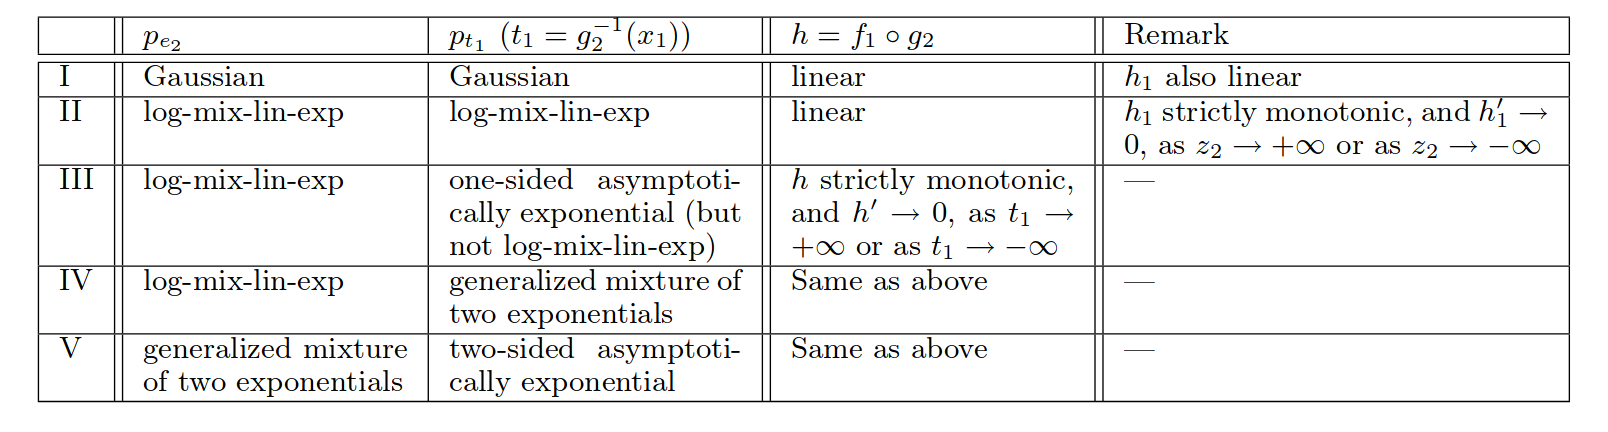
\includegraphics[scale=0.2]{PNL.png}
	\caption{All unidentifiable cases with the assumptions made above}
\end{figure}
\end{frame}

\section{Learning Algorithms}
\subsection{Score Based Method}
\begin{frame}
\frametitle{Learning Algorithms : Score Based Method}
\begin{itemize}
\item The score proposed by \cite{continous} and \cite{nowzohour}:
$$\hat{G} = \mathrm{argmin}_G \sum_{i=1}^n \mathrm{DM}(res_i^{G, \mathrm{RM}}, res_{-i}^{G, \mathrm{RM}}) + \lambda \#\mathrm{edges}$$
\item DM = Dependence Method \hspace{1cm} RM = Regression Method
\item Idea : Noises are independent
\item They do not prove (or even claim) that the minimizing of the above score is a consistent estimator for the correct DAG.
\item Learning Algorithm: Greedy DAG Search or Brute Force (Only for small graphs)
\end{itemize}
\end{frame}

\subsection{RESIT}
\begin{frame}
\frametitle{Learning Algorithms : RESIT Algorithm}
\begin{itemize}
	\item First proposed in \cite{continous}
	\item Assumption : Multivariate ANM + Causal Sufficiency 
	 \item Idea :  $X_i \textrm{ is sink} \iff N_i \bigCI \mathbf{X} \setminus \{X_i\}$ 
	\item The are two stages in the algorithm:
		\begin{itemize}
			\item Stage 1 : Finding a causal order 
			\item Stage 2 : Estimating DAG by removing edges
		\end{itemize}
	\item Number of Tests (Less than PC)
		\begin{itemize}
			\item Stage 1 : $O(n^2)$			
			\item Stage 2 : $O(n)$
		\end{itemize}
\end{itemize}
\end{frame}

\begin{frame}
\frametitle{Learning Algorithms : RESIT Algorithm}
\begin{figure}
	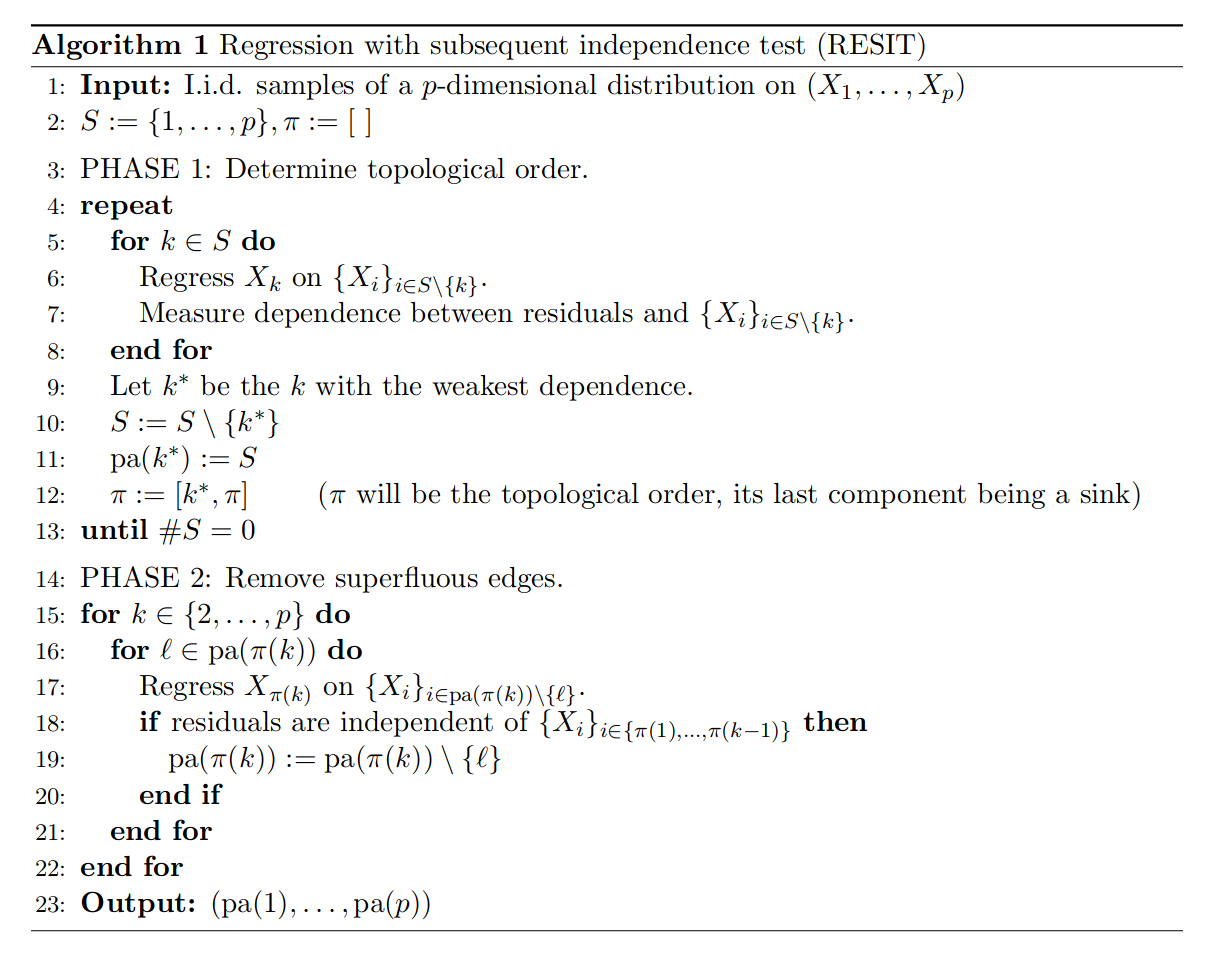
\includegraphics[scale=0.2]{alg.png}
\end{figure}
\end{frame}

\begin{frame}
\frametitle{RESIT Algorithm : Performance (Linear Setting)}
\begin{center}
\scriptsize{$\beta_{jk} \stackrel{}{\sim} [-2,-0.1] \cup [0.1,2]$
$\;\;\;\;\;N_j \stackrel{}{\sim} K_j \cdot \mathrm{sign}(M_j)\cdot |M_j|^{\alpha_j}$
such that
$M_j \stackrel{}{\sim} N(0,1)$, $K_j \stackrel{}{\sim} U(0.1,0.5)$ 
and
$\alpha_j \stackrel{}{\sim} U([2,4])$. }
\end{center}
\begin{figure}[h!]
	\centering
	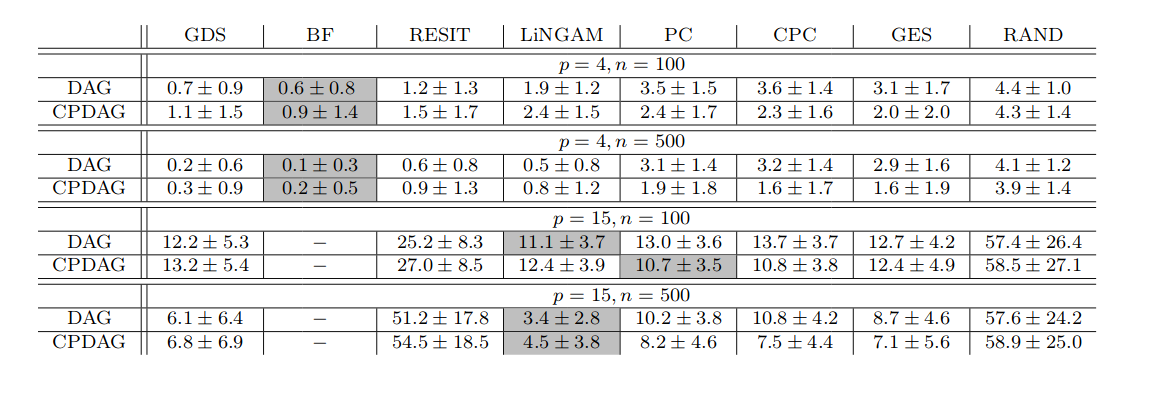
\includegraphics[scale=0.28]{linear.png}
	\caption{Structural Hamming Distance of Estimated Graph}
\end{figure}
\end{frame}

\begin{frame}
\frametitle{RESIT Algorithm : Performance (Non Linear Setting)}
\begin{center}
	\scriptsize{
		Functions sampled from a Gaussian process with $BW=1$. Gaussian Noise with random variance.
	}
\end{center}
\begin{figure}[h!]
	\centering
	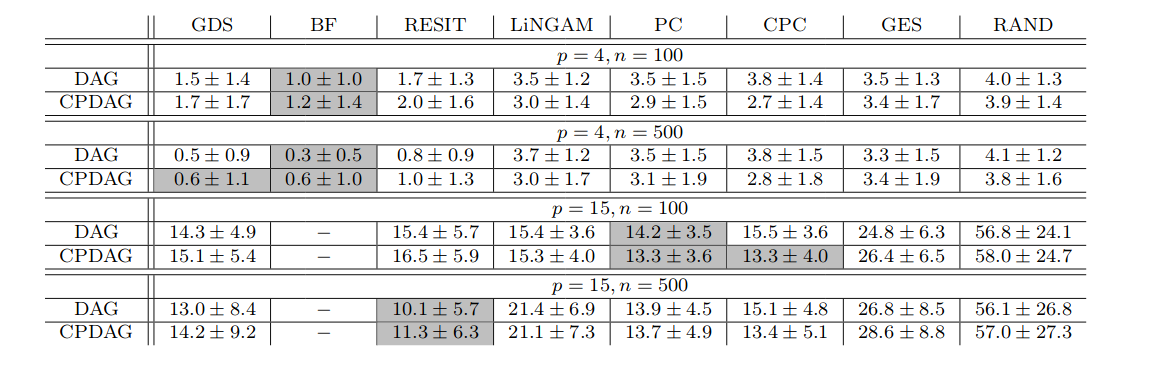
\includegraphics[scale=0.28]{dif.png}
	\caption{Structural Hamming Distance of Estimated Graph}
\end{figure}
\end{frame}

\begin{frame}
Average Temperature, Altitude, Duration of Sunlight from 349 German weather stations.

\begin{figure}[h!]
\frametitle{Real Dataset?}
	\begin{center}
		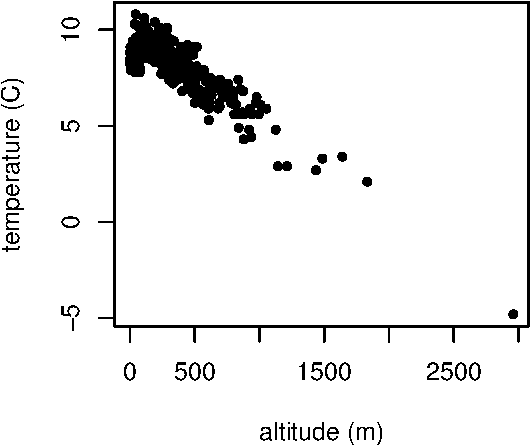
\includegraphics[width=0.31\textwidth]{experimentAltTempcut}
		\hspace{0.02\textwidth}
		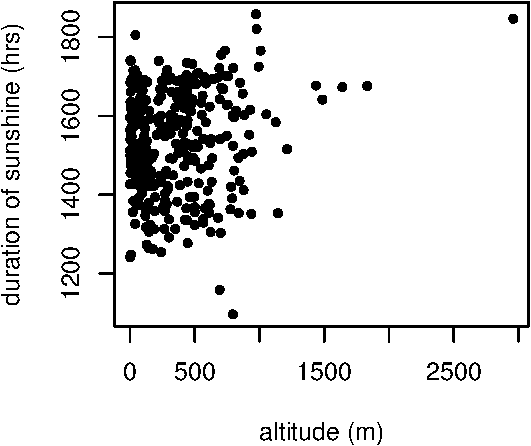
\includegraphics[width=0.31\textwidth]{experimentAltSuncut}
		\hspace{0.02\textwidth}
		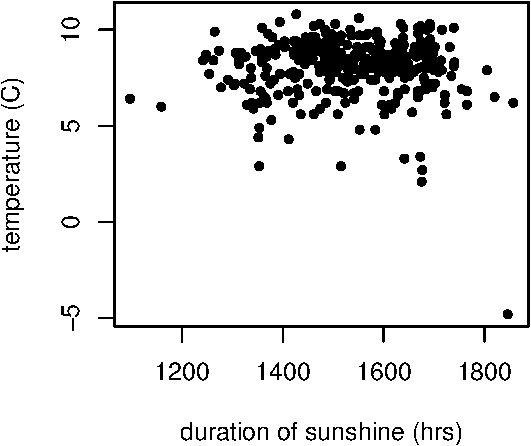
\includegraphics[width=0.31\textwidth]{experimentSunTempcut}
	\end{center}
	\caption{Scatter plot of the data}
	\label{fig:alt}
\end{figure}

\end{frame}
\begin{frame}
\frametitle{Real Dataset!}
Output graph of different algorithms:
\vspace{1cm}
\begin{figure}
	\centering
		\begin{tabular}{| c| c |}
			\hline
			Method & Graph \\
			\hline\hline
			LiNGAM & $T \rightarrow A$ \\
			\hline
			PC &  $T \rightarrow A \leftarrow DS$ \\
			\hline
			CPC& $T \rightarrow A \leftarrow DS$ \\
			\hline
			GDS& $T \leftarrow A \rightarrow DS$\\
			\hline
			BF& $T \leftarrow A \rightarrow DS$\\
			\hline
			RESIT&$T \leftarrow A \rightarrow DS$\\
			\hline
		\end{tabular}
	\end{figure}
\end{frame}

\section{Hidden Variables}
\begin{frame}
\frametitle{Confounder Detection in The Bivariate Case}
\begin{columns}
\begin{column}{0.33\textwidth}
\scriptsize{
	\begin{equation*}
	\begin{cases}
	X = f(T) + N_X\\
	Y = g(T) + N_Y
	\end{cases}
	\end{equation*}
}
\begin{figure}
\begin{tikzpicture}[->,shorten >=1pt,auto,node distance=1.5cm,
thick,main node/.style={circle,draw,font=\sffamily\large\bfseries}]
\node[main node] (x) {X};
\node[main node] (y) [right of=x] {Y};
\path[every node/.style={font=\sffamily\small}]
(x) edge node [right] {} (y);
\end{tikzpicture}
\end{figure}
\begin{figure}
\begin{tikzpicture}[->,shorten >=1pt,auto,node distance=1.5cm,
thick,main node/.style={circle,draw,font=\sffamily\large\bfseries}]
\node[main node] (w) {T};
\node[main node] (x) [below left of=w] {X};
\node[main node] (y) [below right of=w] {Y};
\path[every node/.style={font=\sffamily\small}]
(w) edge node [left] {} (x)
(w) edge node [left] {} (y);
\end{tikzpicture}
\end{figure}
\begin{figure}
\begin{tikzpicture}[->,shorten >=1pt,auto,node distance=1.5cm,
thick,main node/.style={circle,draw,font=\sffamily\large\bfseries}]
\node[main node] (x) {X};
\node[main node] (y) [right of = x]{Y};
\path[every node/.style={font=\sffamily\small}]
(y) edge node [left] {} (x);
\end{tikzpicture}
\end{figure}

\end{column}

\begin{column}{0.67\textwidth}
\scriptsize{
\underline{Naive Method: Dimension Reduction}
$$\hat{T}_k = \mathrm{argmin}_{t\in[0,1]} ||(X_k, Y_k) - \mathbf{s}(t)||_2$$ find $\hat{\mathbf{s}}$ that minimizes 
$\sum^n_{k=1} ||(X_k, Y_k) - \mathbf{s}(\hat{T}_k)||_2$. Then test the independence of noise variables}
\begin{figure}
	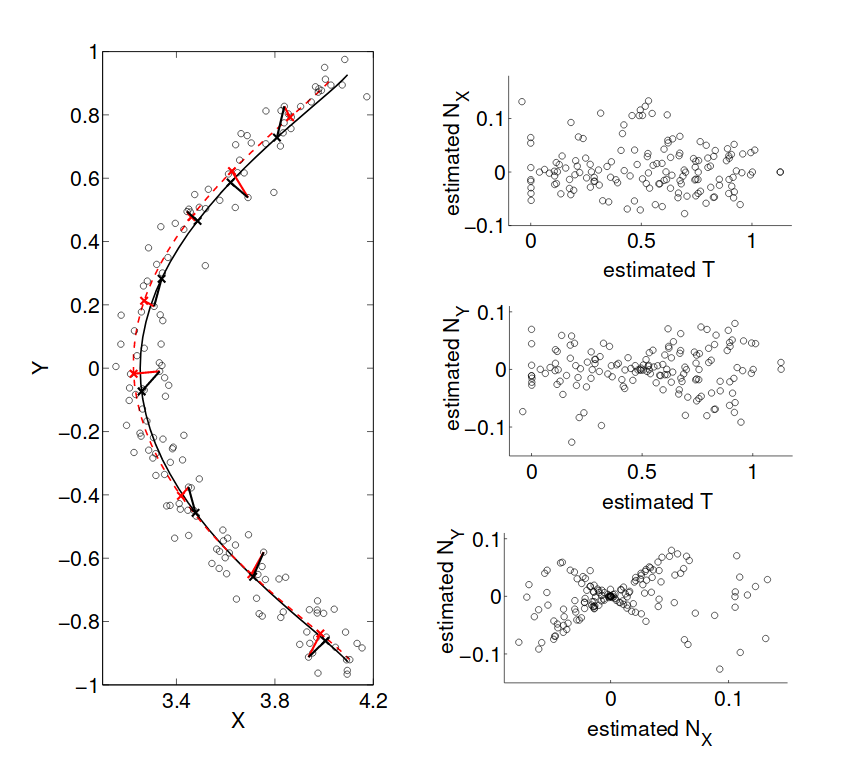
\includegraphics[scale = 0.17]{dimred.png}
\end{figure}
\end{column}
\end{columns}
\end{frame}
\subsection{ICAN}
\begin{frame}
\frametitle{Confounder: ICAN Algorithm}
\begin{columns}
\begin{column}{0.5\textwidth}
	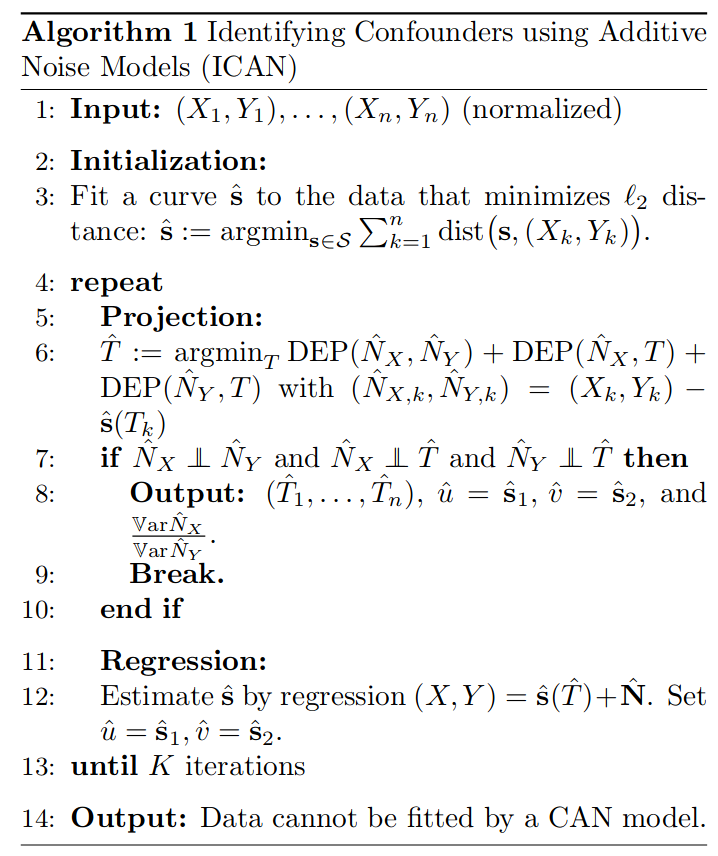
\includegraphics[scale=0.25]{ican.png}
\end{column}
\begin{column}{0.5\textwidth}
	\begin{itemize}
		\item The Naive method does not work even in simple cases.
		\item ICAN was first introduced in \cite{confounder}.
		\item Idea: Minimizing dependence instead of the $l_2$ norm.
		\item Proof of consistency only for the low noise regime. The algorithm seems to work in large noise regime as well.
	\end{itemize}
\end{column}
\end{columns}
\end{frame}
\section{Time Series}
\subsection{TiMINo}
\begin{frame}
\frametitle{Time Series : TiMINo}
\begin{definition} \label{def:timino}
	Consider a time series $\X_t=(X^i_t)_{i \in V}$. We say the time series satisfies a \emph{TiMINo} if there is a $p>0$ and if $\forall i \in V$ there are sets $\PA[i]{0} \subseteq X^{V\setminus\{i\}}, \PA[i]{k} \subseteq X^V$, s.t. $\forall t$
	%\begin{equation} \label{anm}
	%X^j_t = \sum_{\tau=1}^p \sum_{i \in U} f_{i,\tau}(X_i(t-\tau)) + \eps_j(t)\,, \qquad U \subset V\,,
	%\end{equation}
	%where not all $f_{i,\tau}\equiv \mathrm{const.}$.
	\begin{align} \label{anm}
	X^i_t = f_{i}\big((\PA[i]{p})_{t-p}, \ldots, (\PA[i]{1})_{t-1}, (\PA[i]{0})_{t}, \eps^i_t\big)\,,
	\end{align}
	with  
	%If $f_{j,i}$ is not constant in component $X^{i}_{t-h}$ we draw an arrow from $X^{i}_{t-h}$ to $X^j_t$ in the full time graph 
	$\eps^i_t$ (jointly) independent and for each $i$, $\eps^i_t$ identically distributed in $t$ and the full time graph is acyclic.
\end{definition}
\cite{time}
\end{frame}

\begin{frame}[fragile]
	\frametitle{Time Series : TiMINo}
\begin{figure}
	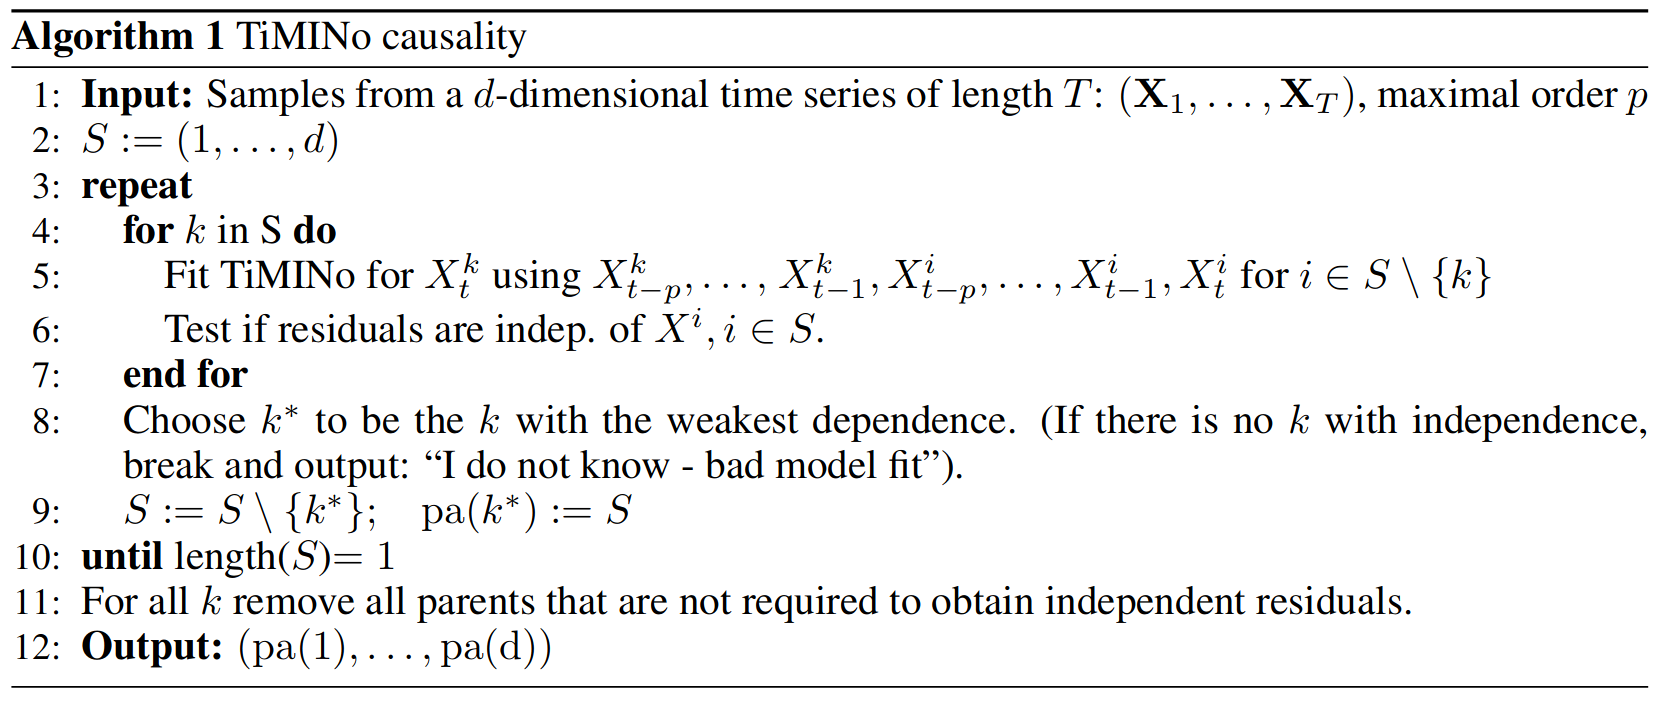
\includegraphics[scale=0.2]{timinoalg.png}
\end{figure}
TiMINo causality has to be provided with a fitting method.
e.g. VAR fitting,  generalized additive models (gam) and  GP regression. 
\end{frame}

\begin{frame}
\frametitle{Time Series : Granger Causality vs. TiMINo}
\begin{itemize}
\item TiMINo allows instantaneous effects.
\item Shifted Time Series ($\tilde{X}_t^i = X_{t-l_i}^i$) \hspace{0.5cm} for example in fMRI Data.  There might be causal relations backwards in time and Granger Causality might fail in these cases. In TiMINo, the summary graph is identifiable.
\item in some cases, TiMINo output is "Can't Decide"
\end{itemize}
\end{frame}



\begin{frame}
\begin{itemize}
\item a simple case with confounder:
\begin{figure}
	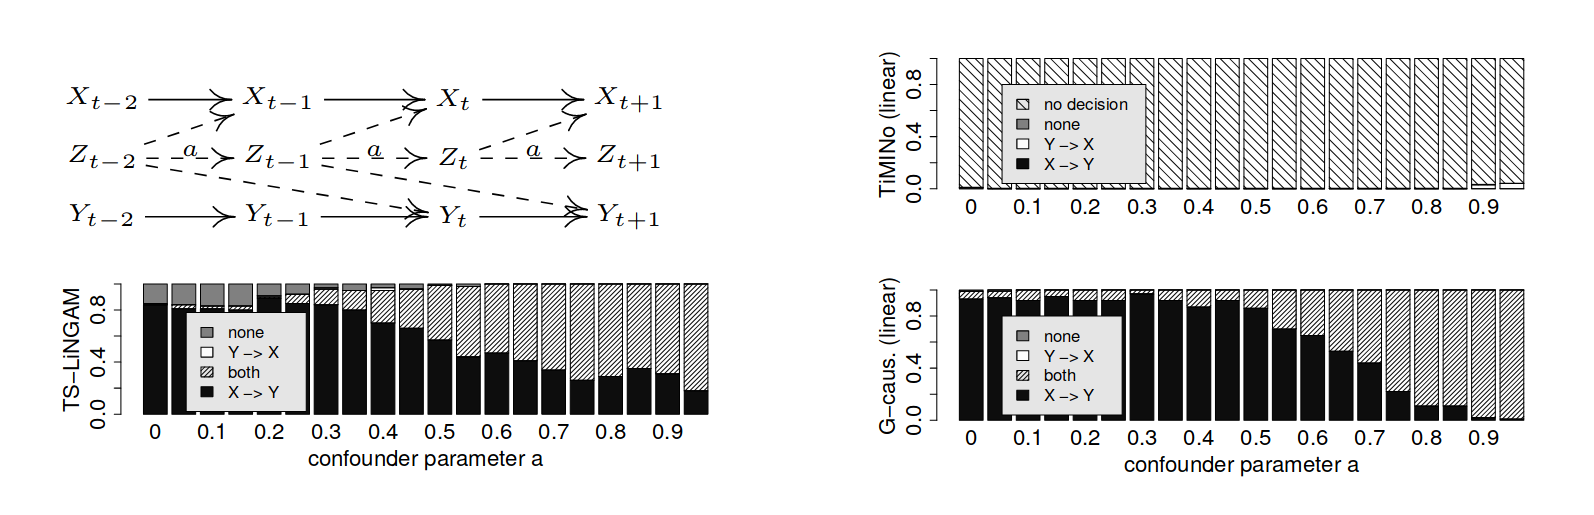
\includegraphics[scale=0.21]{timino.png}
\end{figure}

\item
\tiny{
\begin{equation*}
\begin{cases}
X_t=0.8 X_{t-1} + 0.3 \eps_{X,t}\\
Y_t=0.4 Y_{t-1} + (X_{t-1}-1)^2 +0.3\eps_{Y,t}\\
Z_t=0.4 Z_{t-1} + 0.5 \cos(Y_{t-1}) + \sin(Y_{t-1}) +0.3\eps_{Z,t}
\end{cases}
\end{equation*}
\begin{figure}
	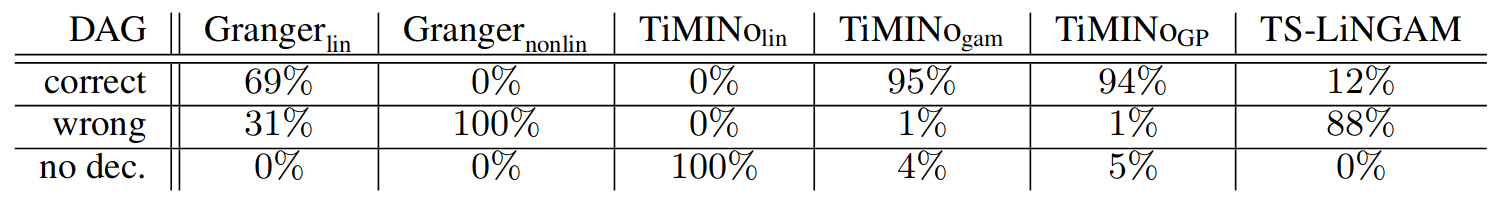
\includegraphics[scale=0.2]{nonlin.png}
\end{figure}
}
\end{itemize}
\end{frame}
\section{Refrences}
\begin{frame}
\frametitle{References}
\scriptsize{
\bibliographystyle{plainnat}
\bibliography{bib}
}
\end{frame}

\end{document}
